\scanpage{54}

c) \deleted{\unsure{Soient|Soit}} $B$ un autre faisceau abélien. Supposons comme dans a) que \deleted{\unsure{le}} $\underline{\operatorname{Hom}}_{\unsure{\mathrm{gr}|u}}(A,G)=0$. Alors on trouve que \unsure{la|le} \begin{tabular}[b]{@{}c@{}}\inserted{catégorie}\\[-2pt]\begin{tikzpicture}[x=1em,y=1em]\draw (0,0)--(.18,.25)--(.36,0);\end{tikzpicture}\\[-4pt]\deleted{\unsure{foncteur|fonction}}\end{tabular} \deleted{\unsure{actuel|est nulle}} $\underline{\operatorname{BIEXT}}(A,B;G)$ est discrète et
\[
\deleted{\operatorname{Biext}(A,B;G)\longleftarrow}
\]
\[
\operatorname{Biext}(A,B;G)\xrightarrow{\sim}\operatorname{Hom}_{\unsure{\mathrm{gr}|u}}\bigl(B,\overset{\substack{\inserted{A^{\prime}}\\\text{\begin{tikzpicture}[x=1em,y=1em]\draw (0,0) .. controls (.08,.19) and (.22,.25) .. (.28,.14) .. controls (.32,.09) and (.28,.02) .. (.22,0);\end{tikzpicture}}}}{\underline{\operatorname{Ext}}}(A,G)\bigr)
\]
d) \begin{tikzpicture}[baseline=-.3ex,x=1em,y=1em]\draw (0,.05) .. controls (-.05,-.08) and (.45,-.08) .. (.7,-.04);\fill (.43,.2) circle (.035);\end{tikzpicture}
\[\inserted{
\operatorname{Biext}(A,B;G)\simeq H^0(S,\underline{\operatorname{Biext}}(A,B;G))\simeq\underline{\operatorname{Hom}}_{\unsure{\mathrm{gr}|g|q}}(B,\underline{\operatorname{Ext}}(A,G))
}\]

Si on suppose $\simeq$ que \deleted{\unsure{Biext}} $\underline{\operatorname{Hom}}_{\unsure{\mathrm{pct}|\mathrm{pet}|\mathrm{fct}}}(A,G)=0$, on trouve
\diagram{\begin{tikzcd}[ampersand replacement=\&,column sep=small,row sep=large]
 \& \& \operatorname{Hom}_{\deleted{\unsure{\mathrm{gr}|\mathrm{ens}}}\,\mathrm{ens}}(B,R^1f_*(G_A)) \arrow[dl] \arrow[d,phantom,"\rotatebox{90}{$\simeq$}" description] \\
\operatorname{Biext}(A,B;G) \arrow[r,hook] \& \operatorname{Hom}_{\mathrm{gr}}(B,R^1f_*(G_A)) \arrow[r,hook] \& H^0(B,R^1f_{B*}(G_{A\times_S\unsure{B}}) \\
 \& \deleted{\unsure{R}\,\unsure{f_*(G_A)}} \& \Vert
\end{tikzcd}}
\begin{flushright}
\begin{tabular}{@{}c@{\quad}c@{\quad}l@{}}
 & & classes de $G_{A\times_S B}$-torseurs \\
 & & \deleted{\unsure{bi\illegible{1}}} \\
 & & \deleted{\unsure{foncteurs}} \\
\begin{tabular}{@{}l@{}}
$=$ classes de $G_{A\times_S B}$-torseurs \\
rigidifiables par \\
$e_A\times_S B$
\end{tabular}
&
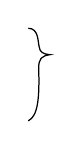
\begin{tikzpicture}[x=0.6cm,y=0.5cm,baseline=0]
\draw[line width=0.45pt] (0,0.85) .. controls (0.22,0.85) and (0.20,0.52) .. (0.23,0.38) .. controls (0.25,0.24) and (0.30,0.20) .. (0.46,0.18) .. controls (0.28,0.15) and (0.22,0.08) .. (0.22,-0.16) .. controls (0.24,-0.95) and (0.20,-1.38) .. (0,-1.50);
\end{tikzpicture}
&
\begin{tabular}{@{}l@{}}
rigidifiés \unsure{par.|p.r.} \\
\unsure{rapp|v.gr.} : $e_A\times_S B$
\end{tabular}
\\
 & & $\rotatebox{-90}{$\hookrightarrow$}$ \\
 & & $H^{\unsure{\text{\rlap{$\scriptstyle0$}$\scriptstyle1$}|1|0}}(A\times_S B,G_{A\times_S B})$
\end{tabular}
\end{flushright}

\diagram{\begin{tikzcd}[ampersand replacement=\&]
A \arrow[r,dash] \arrow[d,dash,"f"'] \& A\times_S B \arrow[d,dash,"f_B"] \\
S \arrow[r,dash] \& B
\end{tikzcd}}

Les torseurs sur $A\times_S B$ \deleted{\unsure{qui}} de gr $G_{A\times_S B}$ \unsure{qu'on obtient|qui désirés|qui désirons} \unsure{sont} ceux qui \begin{tabular}[b]{@{}c@{}}\inserted{a)}\\[-2pt]\begin{tikzpicture}[x=1em,y=1em]\draw (.08,0)--(.36,.55);\end{tikzpicture}\end{tabular} sont $e_A\times_S B$ rigidifiables; et pour lesquels l'application $B\mathbin{-}R^1f_*(G_A)$ qui le définit a deux vertus: b) c'est additif c) ça se factorise par
\[
\deleted{\unsure{R^1f_*}}.\quad\underline{\operatorname{Ext}}(A,G)\simeq A'.
\]
\margin{\begin{tabular}{@{}c@{\quad}l@{}}
\uline{Prop} & Les conditions a) et c) ensemble \\
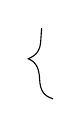
\begin{tikzpicture}[x=0.5cm,y=0.4cm,baseline=0]
\draw[line width=0.4pt] (0.34,1.18) -- (0.32,0.82) .. controls (0.31,0.48) and (0.22,0.33) .. (0,0.21) .. controls (0.23,0.10) and (0.28,-0.16) .. (0.29,-0.45) .. controls (0.30,-0.79) and (0.40,-0.98) .. (0.63,-1.06);
\end{tikzpicture}
& \begin{tabular}{@{}l@{}}
signifient que l'hom \\
$A\unsure{\mathbin{-}|\longrightarrow}R^1\unsure{q|g}_*(G_B)$ est additif
\end{tabular}
\end{tabular}}

\begin{tabular}[b]{@{}l@{}}\inserted{Notons d'ailleurs que la condition a) implique}\\[-2pt]\deleted{\unsure{Supposons qu'on ait également}}\end{tabular} que $L$ est \uline{\unsure{birigidifiable|birigidifiables}} p.r. à $e_A,e_B$, et on trouve des foncteurs \uline{pl. fid.} de catégories discrètes
\diagram{\begin{tikzcd}[ampersand replacement=\&,column sep=small]
\operatorname{BIEXT}(A,B;G) \arrow[r] \& \operatorname{TORS}\,\unsure{\operatorname{BIRIG.}|\operatorname{BRig.}}_{e_A,e_B}(A,B;G) \arrow[r] \& \unsure{\operatorname{TORS}}\,\operatorname{RIG}_{e_A\times_S B}(G_{A\times_S\unsure{B}}
\end{tikzcd}}

La description \begin{tabular}[b]{@{}l@{}}\inserted{en termes du}\\[-2pt]\begin{tikzpicture}[x=1em,y=1em]\draw (0,0) .. controls (.05,.45) and (1.7,.1) .. (2,.6);\end{tikzpicture}\\[-9pt]\deleted{\unsure{par le terme du|par le foncteur du|par $G$ torseurs de}}\end{tabular} milieu est parfois préférable, car a) il est \deleted{\unsure{plus|par}} symétrique en $A,B$, b) dans des cas importants, la pr. flèche est $\eqsim$ une équivalence de catégories.

\margin{53}
